\chapter{Sekventielt henfald}
\label{cha:sekventielt-henfald}
I dette afsnit præsenteres den sekventielle henfaldsmodel, hvorefter der foretages kinematiske
beregninger, der illustrerer hvilket energispektrum dette vil give anledning til. Dette efterfølges
af eksperimentelle resultater, der benyttes til at afgøre om henfaldet foregår ved denne process.  

\section{Teoretisk baggrund}
\label{sec:sekventiel-teo}

Med sekventielt henfald menes henfald fra den populerede tilstand i \Carb til en tilstand i \Be samt
en $\alpha$-partikel. Dette vil give et meget anderledes spektrum end et direkte henfald fra \Carb til
tre $\alpha$-partikler, som giver andledning til et kontinium af tilstande, der afgøres af vinklen mellem
de enkelte $\alpha$-partikler, se \cite{Becker}.

\fxfatal{Indfør primære og sekundære henfald}
Istedet vil det sekventielle give anledning til en smal top ved energien svarende til henfald
grundtilstanden.
\begin{equation}
  \label{eq:alpha0}
  \Carb* \rightarrow \Be(0^{+}) + \alpha_{0}
\end{equation}
% Beryllium-8 er også ustabilt med en bredde $\Gamma = \SI{6.8}{\eV}$, hvilket vil bidrage til bredden
% af toppen, men det primære bidrag vil være detektorens opløsningsevne.
På trods af at beryllium-8 er ustabilt er grundtilstanden stadig ret smal med en bredde på kun
\SI{6.8}{\eV}. Derfor vil bredden af toppen primært skyldes detektorens opløsningsevne. 

Ved de protonenergier, der arbejdes med, så er der endvidere mulighed for at henfalde til den første
exiterede tilstand, der ligger ved \SI{2.95}{\MeV}.
\begin{equation}
  \label{eq:alpha0}
  \Carb* \rightarrow \Be*(2^{+}) + \alpha_{1}
\end{equation}
Bredden af denne top afgøres primært af bredden af beryllium tilstanden, som er
\SI{1.5}{\MeV}. Toppen vil derfor svare til en Gauss fordeling, der er væsenlig breddere, samt ligger
ved lavere energi end den for $\alpha_{0}$.

Idet begge berylliumtilstande er ustabile vil der, pga. den lave levetid, forekomme endnu et henfald
udmiddelbart efter. Dette vil være endnu et alphahenfald, hvormed beryllium kernen splittes op i to
sekundære $\alpha$-partikler, hhv. $\alpha_{21}$ og $\alpha_{22}$. Energien af disse kan bestemmes ud fra følgende
kinematiske overvejelser.

\subsection{Kinematik}
\label{sec:sekv-kinematik}

En skitse af situationen efter det sekundære henfald ses på \cref{fig:secundary}.
\begin{figure}[h]
  \centering
  \includegraphics{Sekventiel-kinematik}
  \caption{Skitse af situationen af det sekundære henfald. Vektorerne angiver hastighederne. $\phi$ er
    vinklen mellem hastigheden af beryllium og de sekundære alphaer i CM for beryllium. $\phi_{2i}$ er
    de tilsvarende vinkler i LAB-systemet.}
  \label{fig:secundary}
\end{figure}

Ud fra energi og impulsbevarelse ses, at energien af de to primære henfaldsprodukter må være
\begin{equation}
  \label{eq:Ealpha0}
  E_{\alpha_{0}} = \frac{2}{3} Q_{1} \qquad E_{\ce{Be}} = \frac{1}{3} Q_{1},
\end{equation}
hvor $Q_{1}$ er den frigivne energi ved det primære henfald. Energien af de to sekundære $\alpha$'er, i CM
for beryllium, kan tilsvarende ud fra bevarelseslovene
\begin{equation}
  \label{eq:Ealpha2}
  E_{\alpha_{2}}' = \frac{1}{2} Q_{2},
\end{equation}
hvor $Q_{2}$ er den tilsvarende energi for det sekundære henfald. Hermed ses tydeligt, at i CM er
energien af de forskellige partikler konstant uanset vinklen.

De tilsvarende størrelser i LAB systemet, kan bestemmes ved at tage højde for tyngdepunktets
bevægelse, som svarer til berylliumkernens bevægelse. Dermed reducerer det til
\begin{align}
  E_{\alpha_{2}} %&= \frac{1}{2}m_{\alpha} (\mvec{V_{\ce{Be}}} + \mvec{V_{\alpha}})^{2} \notag \\
           &= \frac{1}{2}m_{\alpha} (V_{\ce{Be}}^{2} + V_{\alpha}^{2} + 2V_{\ce{Be}}V_{\alpha} \cos \phi) \notag \\
           &= \frac{Q_{1}}{6} + \frac{Q_{2}}{2} + \sqrt{\frac{Q_{1}Q_{2}}{3}} \cos \phi,           
           \label{eq:E2LAB} 
\end{align}
hvor der er anvendt approksimationen $m_{\ce{Be}} = 2m_{\alpha}$.

Ud fra dette ses, at for en stråle af protoner med 2\MeV energi, så vil energien af de to sekundære
$\alpha$-partikler udgøre et kontinium inden for intervallet $E_{\alpha_{2}} = E_{0} \pm \Delta E$. For henfald til
grundtilstanden vil det udgøre energierne mellem ca. \SI{1.2}{\MeV} og \SI{2.35}{\MeV}, hvor henfald
til den exciterede tilstand giver andledning til energier mellem \SI{14}{\keV} og og \SI{5.5}{\MeV}.

Den præcise distribution vil afhænge af distributionen af $\cos \phi$, hvilket er bestemt af de populerede
tilstandes impulsmoment. 

Endvidere er det muligt at bestemme vinklen i LAB-systemet ud fra vinklen i CM og Q-værdierne. Dette
kan udledes trigometrisk ud fra \cref{fig:secundary}, men er ikke medtaget her. Resultatet af dette
er
\begin{equation}
  \label{eq:sekv-vinkel}
  \tan \phi_{2i} = \frac{\sin \phi}{\cos \phi \pm \sqrt{\frac{Q_{1}}{3Q_{2}}}}, i = 1,2 
\end{equation}
Det ses, at som forventet, at maksimale vinkel fremkommer, når CM-vinklen er 90\degree, svarende til
at al energien tilføres den transversale bevægelse. 

\section{Data og databehandling}
\label{sec:sek-data}

\subsection{Koincidens}
\label{sec:koincidens}
For at grovsortere data for protonhændelser, så var det logiske kredsløb indstillet til \lAND,
således at der kun forekom en hændelse, når begge de runde detektorer blevt ramt. Der kan dog
stadigvæk forekomme tilfældige koincidenser. Arbejdet bestod derfor i at bestemme de sande
koincidenser.

Var der i en given hændelse var tre eller flere detekterede partikler, så blev der ledt efter
tripelkoincidenser. Disse kan forekomme på to måder i detektorerne. Enten vil partiklerne have ramt
hver sin detektor eller også vil to have ramt den samme, hvor den tredje så har ramt sin
detektor. Hvis den samlede energi af en sådan triplet er lig med Q-værdien, så er det formentlig et
sæt af tre matchende alphaer. 

Hvis spektret er meget rent, er det også muligt at benytte dobbelkoincidenser. Hvis der i en enkelt
hændelse kun er detekteret to partikler, så er de formentlig to tredjedele af en triplet. Energien
af den sidste er så differencen mellem Q-værdien og den samlede energi af de detekterede
partikler. Det er en afvejning af disse skal tages med. De øger antallet af detekterede koincidenser
kraftigt, men samtidig giver de også andledning fejl. Nogle åbenlyse fejl, såsom at tjekke om
energien af den tredje bliver negativ, opfyldelse af impulsbevarelse kan afhjælpe nogle af
problemerne.

På trods af denne matching forekom, der stadig støj i spektret. Støjen var dog så lokaliseret og
placeret ved ikke kritiske energier, så det var muligt blot at udelade disse energier.


\subsection{Energispektrum}
\label{sec:energispektrum}


\begin{figure}[h!]
  \centering
  \subtop[Dobbelkoincidenser]{\includegraphics[width=0.46\columnwidth]{1077-spec-D}}%
  \hfill
  \subtop[Trippelkoincidenser]{\includegraphics[width=0.46\columnwidth]{1077-spec-T}}%
  \caption{Antal tællinger som funktion af energien for henfald fra \SI{17.8}{\MeV}. Den smalle
    $\alpha_{0}$ og den brede $\alpha_{1}$ top ses tydeligt. Energierne ml. 1400 og 1660\keV er ikke medtaget
    i dobbelkoincidenser. }
  \label{fig:alphaSpectrum}
\end{figure}

På \cref{fig:alphaSpectrum} ses alphaspektret i CM for hhv. dobbelt- og trippelkoincidenser, hvor
der er benyttet 2\MeV protoner. Dette populerer en exciteret $0^{+}$ tilstand med en excitations
energi på \SI{17.8}{\MeV}. Idet $\alpha$-henfald bevarer både impulsmoment og paritet, kan henfaldet
foregå både til grundtilstanden og den exciterede tilstand i beryllium.

Først og fremmest skal det nævnes, at hvis energien af en af de detekterede $\alpha$-partikler lå mellem
1400 og 1660\keV, så er disse ikke medtaget i dobbelkoincidenserne, da dette gav anledning til
støj. Det samme gør sig gældende for trippelkoincidenserne mellem 1460 og 1560\keV.

I toppen af begge spektrer ses tydeligt en smal top omkring 7\MeV. Under denne ligger der en bred
gauss lignende top centreret omkring 5\MeV. Disse toppe stemmer fint overens, både mht. bredde og
energi, med hvad det forventes for $\alpha_{0}$ og $\alpha_{1}$. $\alpha_{1}$-toppen er dog ikke perfekt gaussisk,
hvilket bla. kan forklares ved at der forekommer en bidrag fra de sekundære partikler. Fordelingen
af disse er det dog ikke muligt at sige noget videre meningsfuldt om. Dette kan skyldes støj fra
protonstrålen jvf. diskussion i \cref{cha:rutherford}. \fxfatal{Sørg for at denne reference giver mening.}

De målte spektrum er dermed i overenstemmelse med hypotese om et sekventielt henfald til tre
$\alpha$-partikler via \Be. Det essentiele spørgsmål er så, om det er muligt at stole på de to
spektre.

Ud fra diskutionen i \cref{sec:sekv-kinematik} især med \cref{eq:Ealpha2} og \cref{eq:sekv-vinkel}
i mente, så ses at energien til rådighed for de sekundære $\alpha$-partikler i den transversale retning
afhænger af Q-værdien af det sekundære henfald.

Et henfald fra tilstanden af beryllium til tre alphaer frigøre cirka 90\keV, hvorimod et henfald fra
den exciterede tilstand frigøre omkring 3\MeV. Dette betyder, at den transversale komposant af
hastigheden af de sekundære alphaer er mange gange større, hvilket betyder at vinklen mellem de to
sekundære alphaer kan være tilsvarende større. Benytter man \cref{eq:sekv-vinkel}, så er den
maksimale vinkel \SI{19}{\degree} og \SI{86}{\degree} for hhv. henfald til grundtilstanden og den
exciterede tilstand. 

\fxfatal{Dette skal gennemtænkes.}
Med det benyttede dektorsystem er der ikke fuld dækning i alle retninger, men fordi detektorerne er
placeret symmetrisk, så er detektorerne mere effektive til at detektere hændelser med lille vinkel
mellem de sekundære alphaer, da disse to ofte ville ramme samme detektor. Derimod er sandsynligheden
større for at kun to $\alpha$-partikler bliver detekteret, hvis vinklen er større, da der så er mulighed
for at en af partiklerne slet ikke detekteres.

Hvad betyder dette for koincidensspektrene? Effekten er tydeligst ved dobbeltkoincidenserne. Her
undertrykkes $\alpha_{0}$ kraftigst i forhold til $\alpha_{1}$. Dette skyldes, som beskrevet ovenfor, at der
vil være forholdvis flere hændelser, der skyldes henfald til den exciterede tilstand, hvor \emph{kun} to
partikler detekteres. Ved specifik at vælge disse hændelser undertrykkes dermed $\alpha_{0}$.

Hvorfor er $\alpha_{1}$ så ikke undertrykt i trippelkoincidensspektret? Dette skyldes at der er tale om
en vinkeldistribution, som kan antage alle værdier mellem 0 og maksimalværdien. Dermed vil der
forekomme sekundære partikler fra $\alpha_{1}$ henfald, hvor vinklen er lille. Desuden så er åbningerne
imellem detektorerne i størrelsesorden 20\degree målt fra \target. Dermed er det muligt at begge
sekundære partikler fra $\alpha_{0}$ ikke detekteres, hvorimod der er en sandsynlig for at de sekundære
partikler rammer hver sin detektor, hvis der er tale om $\alpha_{1}$-henfald. Sidst men ikke mindt, skal
det nævnes, at de sekundære alphaer bidrager til $\alpha_{1}$ toppen. 

Den præcise modulering af de to toppe er dermed meget afhængig hvilke koincidensbetingelser der
stilles, men afhænger endvidere også af den specifikke opstilling. For at opnå fuld forståelse af
fordelingen er det derfor nødvendigt at foretage en simulering. Dette ligger dog uden for tidsrammen
af dette projekt. Derfor vil dobbelt- og trippelkoincidenserne behandles separat i den videre
analyse. 

\section{Konklusion}
\label{sec:sekv-konklusion}

Det er vist, at med passende koincidensbetingelser, er det muligt at ekstrahere et samlet
energispektrum, og at dette energispektrum stemmer overens hypotesen om sekventielt
henfald.

Endvidere så er der redegjort for, at forskellen på spektrene for dobbelt- og
trippelkoincidenser skyldes, at disse betingelser udvælger forskellige typer henfald og at denne
selektering afhænger af den specifikke opstilling.  Det må noteres, at spektret ikke er rent nok
til, at fordelingen af de sekundære $\alpha$-partikler kan bestemmes.

% For trippelkoincidenserne har al kinematisk information været tilgængelig, hvorimod
% dobbeltkoincidenserne bygger på antagelsen om et rent spektrum. Dermed må udgangspunktet være at
% trippelkoincidensspektret er det rigtige. 

% På \cref{fig:aSingleSpectrum} ses spektret for de enkelte detektorer for de hændelse, hvor der er
% detekteret to eller flere partikler. Disse spektrer stemmer også overens med hypotesen om
% sekventielt henfald med tydelige $\alpha_{0}$ og $\alpha_{1}$. Begge disse toppe ligger ved energier, hvor der
% ikke kommer forstyrrelser pga. proton beamet, så derfor må det antages at disse skyldes
% $\alpha$-partikler. På baggrund af dette vil jeg argumenterer for, at det samlede spektre underlagt
% koincidensbetigelserne skal stemme overens for de høje energier med de enkelte spektre på
% \cref{fig:aSingleSpectrum}.

% \begin{figure}[b!]
%   \centering
%   \subtop[Detektor 1]{\includegraphics[width=0.42\columnwidth]{1077-spec0}}%
%   \hspace{1cm}
%   \subtop[Detektor 2]{\includegraphics[width=0.42\columnwidth]{1077-spec1}}%
%   \caption{Energispektrum for detektor 1 og 2 for hændelser med to eller flere partikler.}
%   \label{fig:aSingleSpectrum}
% \end{figure}

% \begin{figure}[b]
%   \centering
%   \ContinuedFloat
%   \subtop[Detektor 3]{\includegraphics[width=0.42\columnwidth]{1077-spec2}}%
%   \hspace{1cm}
%   \subtop[Detektor 4]{\includegraphics[width=0.42\columnwidth]{1077-spec3}}%
%   \caption{Energispektrum for detektor 3 og 4 for hændelser med to eller flere partikler.}
% \end{figure}


% Endvidere så er $\alpha$-henfald kraftigt energiafhængige \cite[s. 236]{Martin}, og $\alpha_{0}$ må derfor
% forventes derfor at være den primære henfaldskanal. \fxfatal{Kan man sige det så groft?}
% I forhold til hvor kraftigt $\alpha_{1}$-toppen dominere på \cref{fig:alphaSpectrum}a, så taler dette
% kraftigt imod at dobbelkoincidensspektret svarer til det sande spektrum.

% Spektrene på \cref{fig:aSingleSpectrum} forklarer endvidere, hvorfor fordelingen af de sekundære
% $\alpha$-partikler ikke træder tydeligere frem. Dette skyldes den store mængde resonanser i den lave ende
% af de enkelte spektre. Disse skyldes at prøven indeholder andre elementer end kulstof og beryllium,
% hvilket giver anledning til Rutherfordspredning ved andre energier. Dette problem kan afhjælpes ved
% at benytte en renere prøve, hvor så Rutherfordtoppen fra beryllium skæres væk. 

% \section{Konklusion}
% \label{sec:sekv-konklusion}

% Det kan konkluderes, at spektrene for de enkelte detektorer er i overensstemmelse med hypotesen om
% sekventielt henfald. Endvidere er det også vist at det, med passende koincidensbetingelser, er
% muligt at ekstrahere et samlet energispektrum, og at dette også er i overensstemmelse med
% sekventielt henfald. Det må dog noteres, at de optagne spektre ikke er rene nok til at
% dobbeltkoincidenserne kan benyttes. 











